\documentclass[aspectratio=169,10pt]{beamer}
\usetheme{Madrid}
\usecolortheme{default}
\usepackage{tikz}
\usepackage{booktabs}
\usepackage{fontawesome5}
\usepackage{xcolor}
\usepackage{amsmath}
\usepackage{colortbl}
\usetikzlibrary{arrows.meta,shadows,positioning,fit,shapes.geometric,calc}

% ── palette ──────────────────────────────────────────────────────────
\definecolor{c1}{RGB}{41,128,185}
\definecolor{c2}{RGB}{52,152,219}
\definecolor{c3}{RGB}{155,89,182}
\definecolor{c4}{RGB}{142,68,173}
\definecolor{c5}{RGB}{230,126,34}
\definecolor{c6}{RGB}{211,84,0}
\definecolor{hit}{RGB}{39,174,96}
\definecolor{miss}{RGB}{192,57,43}
\definecolor{warn}{RGB}{243,156,18}

\setbeamercolor{frametitle}{bg=c1,fg=white}
\setbeamercolor{title}{fg=white}
\setbeamercolor{structure}{fg=c1}
\setbeamertemplate{navigation symbols}{}
\setbeamertemplate{footline}[frame number]
\setbeamerfont{frametitle}{series=\bfseries}

% ── confusion matrix cell helpers ────────────────────────────────────
\newcommand{\chit}[1]{\cellcolor{hit!30} #1}
\newcommand{\cmiss}[1]{\cellcolor{miss!25} #1}
\newcommand{\czero}{\cellcolor{black!4} }

\title{\textbf{Graph-Based Vulnerability Retrieval}\\[4pt]}
\subtitle{Master's Thesis — Technical Progress · Checkpoint 2}
\author{Lívia}
\institute{TU Munich · Siemens}
\date{\today}

\begin{document}

% ── title ─────────────────────────────────────────────────────────────
\begin{frame}
\titlepage
\end{frame}

% ── agenda ────────────────────────────────────────────────────────────
\begin{frame}{Agenda}
\begin{columns}[T]
\begin{column}{0.55\textwidth}
  \begin{enumerate}
    \item[\textcolor{c1}{\faIcon{redo}}] \textbf{System recap} —
      pipeline overview \& what this checkpoint covers

    \vspace{0.6em}
    \item[\textcolor{c3}{\faIcon{project-diagram}}] \textbf{Graph slicing} —
      how we fixed the semantic diff and extract $G_{\text{vuln}}$

    \vspace{0.6em}
    \item[\textcolor{c2}{\faIcon{layer-group}}] \textbf{Embedders} —
      structural (NetLSD, WL, GIN, Combined) vs.\ semantic (CodeBERT)

    \vspace{0.6em}
    \item[\textcolor{c4}{\faIcon{chart-bar}}] \textbf{Results} —
      self-retrieval and CWE recall across all embedders ($n = 225$)

    \vspace{0.6em}
    \item[\textcolor{c5}{\faIcon{th}}] \textbf{Confusion matrix} —
      per-CWE retrieval quality \& motivation for knowledge graphs

    \vspace{0.6em}
    \item[\textcolor{hit}{\faIcon{lightbulb}}] \textbf{Key findings \& next steps}
  \end{enumerate}
\end{column}
\begin{column}{0.42\textwidth}
  \begin{block}{Focus of this checkpoint}
    Stages \textbf{III} (vulnerability diff) and \textbf{IV} (graph embedding)
    of the end-to-end pipeline.\\[0.5em]
    Main questions addressed:
    \begin{itemize}
      \item Which embedder best separates CVEs?
      \item Do structural or semantic features cluster CWEs better?
      \item Where do retrievals fail, and why?
    \end{itemize}
  \end{block}
\end{column}
\end{columns}
\end{frame}

% ══════════════════════════════════════════════════════════════════════
\section{Recap}
% ══════════════════════════════════════════════════════════════════════

\begin{frame}{System Recap}
\centering
\resizebox{0.96\textwidth}{!}{%
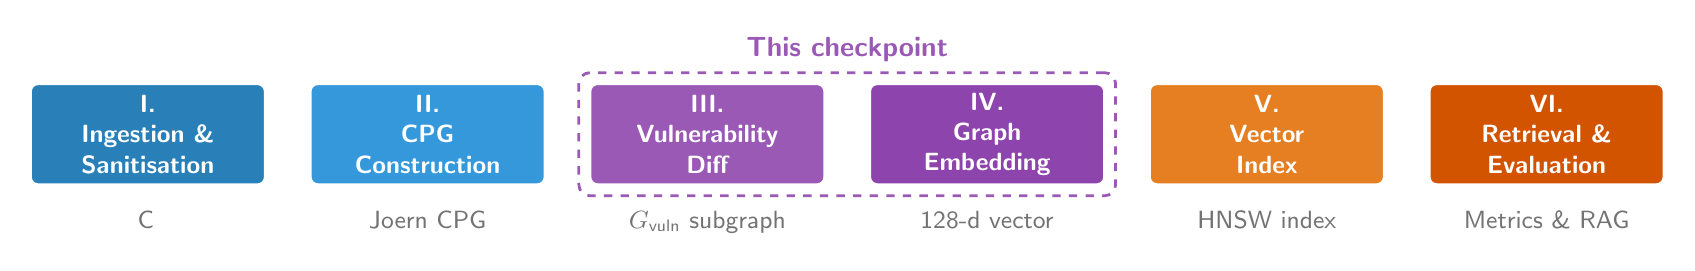
\begin{tikzpicture}[node distance=0pt,
  block/.style={rectangle,minimum width=3.0cm,minimum height=1.3cm,
                text centered,text width=2.7cm,draw=white,line width=1.5pt,
                font=\sffamily\small\bfseries,rounded corners=3pt}]
  \node (n1) [block,fill=c1,text=white] {I.\\Ingestion \&\\Sanitisation};
  \node (n2) [block,fill=c2,text=white,right=0.5cm of n1] {II.\\CPG\\Construction};
  \node (n3) [block,fill=c3,text=white,right=0.5cm of n2] {III.\\Vulnerability\\Diff};
  \node (n4) [block,fill=c4,text=white,right=0.5cm of n3] {IV.\\Graph\\Embedding};
  \node (n5) [block,fill=c5,text=white,right=0.5cm of n4] {V.\\Vector\\Index};
  \node (n6) [block,fill=c6,text=white,right=0.5cm of n5] {VI.\\Retrieval \&\\Evaluation};
  \foreach \i [evaluate=\i as \next using int(\i+1)] in {1,2,3,4,5}{
    \fill[white!30] (n\i.north east) -- ++(0.35,-0.65) -- (n\i.south east)--cycle;
  }
  \foreach \n/\lbl in {
    n1/C\,/\,C++ Source,
    n2/Joern CPG,
    n3/$G_{\text{vuln}}$ subgraph,
    n4/128-d vector,
    n5/HNSW index,
    n6/Metrics \& RAG}{
    \node[below=0.18cm of \n,font=\small\sffamily\color{black!55}] {\lbl};
  }
  \node[draw=c3,dashed,line width=1pt,rounded corners=4pt,
        fit=(n3)(n4),inner sep=3pt,
        label={[font=\sffamily\bfseries\color{c3}]above:This checkpoint}] {};
\end{tikzpicture}}

\vspace{0.8em}
\begin{columns}[t]
  \begin{column}{0.33\textwidth}\centering
    \textbf{\textcolor{c1}{Data Layer}}\\
    \scriptsize 75 original CVEs $+$ 225 augmented (GPT-4o, DeepSeek-R1, LLaMA, o3-mini)
  \end{column}
  \begin{column}{0.33\textwidth}\centering
    \textbf{\textcolor{c3}{Representation Layer} } \\
    \scriptsize Semantic diff $\rightarrow$ latent vector. \textbf{Focus today.}
  \end{column}
  \begin{column}{0.33\textwidth}\centering
    \textbf{\textcolor{c5}{Retrieval Layer}}\\
    \scriptsize ANN search; self-retrieval \& CWE recall evaluated.
  \end{column}
\end{columns}
\end{frame}

% ══════════════════════════════════════════════════════════════════════
\section{Graph Slicing}
% ══════════════════════════════════════════════════════════════════════

\begin{frame}{Graph Slicing: Semantic Diff to $G_{\text{vuln}}$}
\begin{columns}[T]
\begin{column}{0.50\textwidth}

  \textbf{Problem with the old approach}\\[3pt]
  Joern assigns non-deterministic node IDs across runs.
  ID-based diff produced $G_{\text{vuln}} \approx G_{\text{before}}$ —
  all functions appeared structurally identical.

  \vspace{0.9em}
  \textbf{Fix: fingerprint matching by \texttt{(node\_type, CODE)}}\\[3pt]
  \begin{itemize}
    \item \textcolor{miss}{\textbf{Removed}} — node in $G_{\text{before}}$ only
    \item \textcolor{hit}{\textbf{Added}} — node in $G_{\text{after}}$ only
    \item \textcolor{warn!90!black}{\textbf{Context}} — unchanged neighbours\\
          within $n{=}1$ hop on PDG/CDG/CFG edges
  \end{itemize}

  \vspace{0.9em}
  \textbf{Joern wrapper fix}\\[3pt]
  Scaffold boilerplate nodes (injected during export) are now
  stripped before embedding — eliminating shared structural noise.

\end{column}
\begin{column}{0.46\textwidth}
  \centering
  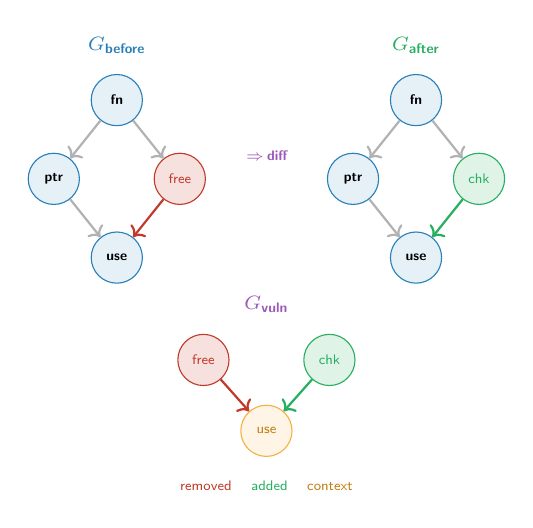
\begin{tikzpicture}[
    fn/.style={circle,draw=c1,fill=c1!12,font=\tiny\sffamily\bfseries,
               minimum size=0.65cm,inner sep=1pt},
    rm/.style={circle,draw=miss,fill=miss!15,font=\tiny\sffamily,
               minimum size=0.65cm,inner sep=1pt},
    ad/.style={circle,draw=hit,fill=hit!15,font=\tiny\sffamily,
               minimum size=0.65cm,inner sep=1pt},
    cx/.style={circle,draw=warn!80,fill=warn!10,font=\tiny\sffamily,
               minimum size=0.65cm,inner sep=1pt},
    lbl/.style={font=\scriptsize\sffamily\bfseries},
    arr/.style={->,thick,black!30}]

    \node[lbl,c1]  at (-1.9, 3.2) {$G_{\text{before}}$};
    \node[fn] (b1) at (-1.9, 2.5) {fn};
    \node[fn] (b2) at (-2.7, 1.5) {ptr};
    \node[rm] (b3) at (-1.1, 1.5) {\textcolor{miss}{free}};
    \node[fn] (b4) at (-1.9, 0.5) {use};
    \draw[arr] (b1)--(b2); \draw[arr] (b1)--(b3);
    \draw[->,miss,thick] (b3)--(b4); \draw[arr] (b2)--(b4);

    \node[lbl,hit]  at (1.9, 3.2) {$G_{\text{after}}$};
    \node[fn] (a1) at (1.9, 2.5) {fn};
    \node[fn] (a2) at (1.1, 1.5) {ptr};
    \node[ad] (a3) at (2.7, 1.5) {\textcolor{hit}{chk}};
    \node[fn] (a4) at (1.9, 0.5) {use};
    \draw[arr] (a1)--(a2); \draw[arr] (a1)--(a3);
    \draw[->,hit,thick] (a3)--(a4); \draw[arr] (a2)--(a4);

    \node[font=\tiny\sffamily\bfseries,c3] at (0, 1.8) {$\Rightarrow$\,diff};

    \node[lbl,c3] at (0, -0.1) {$G_{\text{vuln}}$};
    \node[rm] (v1) at (-0.8, -0.8) {\textcolor{miss}{free}};
    \node[ad] (v2) at ( 0.8, -0.8) {\textcolor{hit}{chk}};
    \node[cx] (v3) at ( 0.0, -1.7) {\textcolor{warn!80!black}{use}};
    \draw[->,miss,thick] (v1)--(v3);
    \draw[->,hit,thick]  (v2)--(v3);
    \node[font=\tiny\sffamily,black!50,align=center] at (0,-2.4)
      {\textcolor{miss}{removed} \quad \textcolor{hit}{added} \quad \textcolor{warn!80!black}{context}};
  \end{tikzpicture}
\end{column}
\end{columns}
\end{frame}

% ══════════════════════════════════════════════════════════════════════
\section{Embedders}
% ══════════════════════════════════════════════════════════════════════

\begin{frame}{Graph Embedders Overview}
\vspace{0.2em}
\centering
{\small
\renewcommand{\arraystretch}{1.3}
\begin{tabular}{llp{5.8cm}l}
  \toprule
  \textbf{Name} & \textbf{Type} & \textbf{What it captures} & \textbf{Note} \\
  \midrule
  \textbf{NetLSD}   & Structural & Heat trace of graph Laplacian. Permutation-invariant; global topology. & Collapses on small graphs \\
  \textbf{WL}       & Structural & Weisfeiler-Lehman colour refinement. Subtree-kernel equivalent. & Node-label aware \\
  \textbf{GIN}      & Structural & 3-layer Graph Isomorphism Net, frozen random weights. & Distance-preserving \\
  \rowcolor{c1!10}
  \textbf{Combined} & Structural & \textbf{NetLSD $\oplus$ WL $\oplus$ GIN} projected via PCA. Not CodeBERT. & Most expressive structural \\
  \textbf{CodeBERT seq}     & Semantic & Mean-pool last-layer activations over the full \texttt{CODE} token sequence. & Ignores graph structure \\
  \textbf{CodeBERT pattern} & Semantic & Per-node CodeBERT embedding, aggregated by node type. & Finer-grained \\
  \bottomrule
\end{tabular}}

% \vspace{0.8em}
% \begin{block}{Note on \textbf{Combined}}
%   \textbf{Combined = NetLSD + WL + GIN} (three structural methods concatenated and PCA-reduced to 128-d).
%   It does \emph{not} include CodeBERT.
%   A GIN $\oplus$ CodeBERT hybrid is a proposed \textbf{next step} — it does not exist yet.
% \end{block}
\end{frame}

% ══════════════════════════════════════════════════════════════════════
\section{Results}
% ══════════════════════════════════════════════════════════════════════

\begin{frame}{Retrieval Results — 225 pairs, $G_{\text{vuln}}$}
\begin{columns}[T]
\begin{column}{0.52\textwidth}

  \textbf{Evaluation protocol}\\[3pt]
  \begin{description}[\textbf{CWE Recall}]
    \item[\textbf{SR@$K$}] Self-retrieval hit@$K$: query each embedding against the full index; fraction that retrieve the correct CVE in top-$K$.
    \item[\textbf{CWE Recall}] Fraction of top-5 neighbours sharing the query's CWE — measures cluster quality, not exact match.
  \end{description}

  \vspace{0.8em}
  {\small
  \renewcommand{\arraystretch}{1}
  \begin{tabular}{lccc}
    \toprule
    \textbf{Embedder} & \textbf{SR@1} & \textbf{SR@5} & \textbf{CWE rec.} \\
    \midrule
    \rowcolor{c1!12}
    Combined          & \textbf{86.3\%} & \textbf{94.5\%} & \textbf{51.9\%} \\
    GIN               & 75.3\%          & 84.9\%          & 39.8\% \\
    CodeBERT seq      & 75.3\%          & 86.3\%          & 41.2\% \\
    CodeBERT pattern  & 71.2\%          & 83.6\%          & 41.5\% \\
    WL                & 67.1\%          & 75.3\%          & 34.8\% \\
    RGCN              & 60.3\%          & 78.1\%          & 37.2\% \\
    NetLSD            & 32.9\%          & 54.8\%          & 21.0\% \\
    \bottomrule
  \end{tabular}}

\end{column}
\begin{column}{0.45\textwidth}

  % SR@1 bar chart
  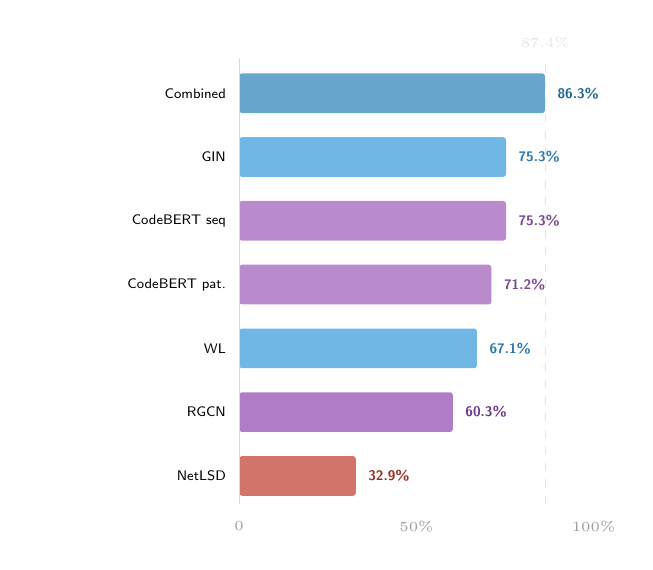
\begin{tikzpicture}[scale=0.9]
    \foreach \y/\lbl/\col/\val/\pct in {
      5.6/{Combined}/c1/0.863/86.3\%,
      4.7/{GIN}/c2/0.753/75.3\%,
      3.8/{CodeBERT seq}/c3/0.753/75.3\%,
      2.9/{CodeBERT pat.}/c3/0.712/71.2\%,
      2.0/{WL}/c2/0.671/67.1\%,
      1.1/{RGCN}/c4/0.603/60.3\%,
      0.2/{NetLSD}/miss/0.329/32.9\%}{
      \node[left,font=\tiny\sffamily,text width=2.4cm,align=right] at (0,\y) {\lbl};
      \fill[\col!70,rounded corners=1pt] (0.05,\y-0.28) rectangle ({0.05+5.0*\val},\y+0.28);
      \node[right,font=\tiny\sffamily\bfseries,\col!80!black]
        at ({0.05+5.0*\val+0.04},\y) {\pct};
    }
    \draw[black!15] (0.05,-0.2)--(0.05,6.1);
    \draw[black!10,dashed] (4.37,-0.2)--(4.37,6.1)
      node[above,font=\tiny\color{black!40}] {87.4\%};
    \node[below,font=\tiny\color{black!40}] at (0.05,-0.3) {0};
    \node[below,font=\tiny\color{black!40}] at (2.55,-0.3) {50\%};
    \node[below,font=\tiny\color{black!40}] at (5.05,-0.3) {100\%};
  \end{tikzpicture}

  \vspace{0.3em}
  {\scriptsize\color{black!55}
  $n = 225$ pairs (75 original + 150 LLM re-implementations).\\
  Self-retrieval: query = index sample (no held-out split).}

\end{column}
\end{columns}
\end{frame}

% ══════════════════════════════════════════════════════════════════════
\section{Confusion Matrix}
% ══════════════════════════════════════════════════════════════════════

\begin{frame}{CWE Retrieval Confusion — Combined Embedder}
\begin{columns}[T]
\begin{column}{0.54\textwidth}
  \centering
  \vspace{0.3em}
  % 7x7 confusion matrix (major CWEs)
  % Rows = query CWE, Cols = top-1 retrieved CWE
  % Data: Combined embedder, n=225, sr top-1
  {\scriptsize
  \renewcommand{\arraystretch}{1.15}
  \setlength{\tabcolsep}{3.5pt}
  \begin{tabular}{r|ccccccc}
    % columns: UAF  NULLPTR  INTOVF  LOCK  RACE  DEAD  MEM
    \textbf{Query \textbackslash\ Retrieved}
      & \rotatebox{60}{\tiny UAF}
      & \rotatebox{60}{\tiny Null Ptr}
      & \rotatebox{60}{\tiny Int Ovf}
      & \rotatebox{60}{\tiny Locking}
      & \rotatebox{60}{\tiny Race}
      & \rotatebox{60}{\tiny Deadlock}
      & \rotatebox{60}{\tiny Mem Leak} \\
    \hline
    \tiny Use After Free      & \chit{12} & \czero 0 & \czero 0 & \czero 0 & \czero 0 & \czero 0 & \czero 0 \\
    \tiny Null Ptr Deref      & \cmiss{ 1} & \chit{ 8} & \czero 0 & \czero 0 & \czero 0 & \cmiss{ 1} & \czero 0 \\
    \tiny Integer Overflow    & \czero 0 & \czero 0 & \chit{10} & \czero 0 & \czero 0 & \czero 0 & \czero 0 \\
    \tiny Improper Locking    & \czero 0 & \czero 0 & \czero 0 & \chit{ 8} & \czero 0 & \czero 0 & \czero 0 \\
    \tiny Race Condition      & \czero 0 & \czero 0 & \czero 0 & \czero 0 & \chit{ 5} & \czero 0 & \czero 0 \\
    \tiny Deadlock            & \czero 0 & \czero 0 & \czero 0 & \czero 0 & \czero 0 & \chit{ 4} & \czero 0 \\
    \tiny Memory Leak         & \czero 0 & \czero 0 & \czero 0 & \czero 0 & \czero 0 & \czero 0 & \chit{ 2} \\
  \end{tabular}}

  \vspace{0.5em}
  {\scriptsize\color{black!55}
  \textcolor{hit!70!black}{\rule{0.8em}{0.8em}} Correct \quad
  \textcolor{miss!70!black}{\rule{0.8em}{0.8em}} Confused.
  Rows: query CWE. Cols: CWE of top-1 retrieved CVE.\\
  Combined embedder, $n=225$, top-7 CWEs shown.}
\end{column}
\begin{column}{0.43\textwidth}

  \textbf{What the matrix tells us}

  \vspace{0.5em}
  \begin{itemize}
    \item \textbf{Strong diagonal} — 90.5\% top-1 retrieval stays within the same CWE class.
    \item \textbf{Semantically coherent confusions} — Null Ptr Deref is confused with UAF and Deadlock, both involving invalid memory/resource access. The errors are \emph{not} random.
    \item \textbf{Hard cases} — Null Ptr Deref (8/11 correct): the patch signature (add a null check) is topologically similar to adding a lock or a free-guard.
  \end{itemize}

  % \vspace{0.7em}
  % \begin{block}{Why this motivates Knowledge Graphs}
  %   \small The off-diagonal errors are \emph{semantically adjacent} CWEs.
  %   A KG that encodes CWE relationships (e.g.\ CWE-476 $\sim$ CWE-416)
  %   could post-rank results: a Null-Ptr miss retrieved as UAF is
  %   \emph{useful}, not random noise.
  % \end{block}
\end{column}
\end{columns}
\end{frame}

% ══════════════════════════════════════════════════════════════════════
\section{Key Findings}
% ══════════════════════════════════════════════════════════════════════

\begin{frame}{Key Findings}
\begin{columns}[T]
\begin{column}{0.48\textwidth}
  \begin{enumerate}
    \item[\faIcon{bug}] \textbf{ID-based diff was fatally flawed.}\\
      Joern IDs are non-deterministic across runs.
      All graphs were indistinguishable.\\
      \textit{Fix: \texttt{(type, CODE)} fingerprint matching.}

    \vspace{0.7em}
    \item[\faIcon{layer-group}] \textbf{Combined is clearly the best structural embedder.}\\
      SR@1 = 86.3\%, CWE recall = 51.9\%.
      Concatenating all three structural signals (NetLSD + WL + GIN)
      outperforms each individually.

    \vspace{0.7em}
    \item[\faIcon{compress-arrows-alt}] \textbf{NetLSD collapses on small graphs.}\\
      Effective dimension $\approx 1$; pairwise cosine $> 0.99$.
      Cannot be used as sole embedder on $G_{\text{vuln}}$ subgraphs.
  \end{enumerate}
\end{column}
\begin{column}{0.48\textwidth}
  \begin{enumerate}
    \item[\faIcon{code}] \textbf{Structural and semantic signals are complementary.}\\
      GIN (structural) and CodeBERT (semantic) achieve the same SR@1 (75.3\%)
      but differ on CWE recall (39.8\% vs.\ 41.2\%).
      Neither dominates; a hybrid is the natural next step.

    \vspace{0.7em}
    \item[\faIcon{project-diagram}] \textbf{Errors are semantically coherent.}\\
      90.5\% of top-1 retrievals stay within the correct CWE.
      Confusions occur between structurally similar patch patterns
      (e.g.\ null-check $\approx$ lock-guard).
      This justifies knowledge-graph-based re-ranking.

    \vspace{0.7em}
    \item[\faIcon{exclamation-triangle}] \textbf{Self-retrieval is a lower bound.}\\
      No held-out query split yet.
      True generalisation performance is unknown.
  \end{enumerate}
\end{column}
\end{columns}
\end{frame}

% ══════════════════════════════════════════════════════════════════════
\section{Next Steps}
% ══════════════════════════════════════════════════════════════════════

\begin{frame}{Next Steps}
% \begin{columns}[T]
% \begin{column}{0.60\textwidth}

  \textbf{1. Hybrid structural + semantic embedding}\\[2pt]
  Build a \texttt{HybridEmbedder} that concatenates GIN (graph topology)
  with CodeBERT (code semantics) into a single 128-d vector.
  GIN captures \emph{what changed structurally}; CodeBERT captures
  \emph{what the code means}. The confusion matrix shows they fail
  in different places.

  \vspace{0.8em}
  \textbf{2. Semantic graph diff for $G_{\text{vuln}}$}\\[2pt]
  Current diff uses exact string match on \texttt{CODE} fields — it
  misses rewrites that change logic while keeping function signatures.
  New approach: embed each node's code with CodeBERT and flag nodes
  whose embedding distance exceeds a threshold. Detects logical
  changes invisible to string comparison.

  \vspace{0.8em}
  \textbf{3. Held-out evaluation set}\\[2pt]
  Self-retrieval is circular — the query is always in the index.
  Need a genuinely unseen query set: real-world bug reports or
  cross-version CVE matches with known ground-truth targets.
  This gives honest precision/recall numbers for the thesis.

% \end{column}
% \begin{column}{0.36\textwidth}

%   \vspace{0.5em}
%   \begin{block}{Target metrics (next checkpoint)}
%     \centering\small
%     SR@1 $\geq 90\%$ (hybrid)\\[3pt]
%     CWE Recall $\geq 60\%$\\[3pt]
%     Held-out Hit@5 $\geq 50\%$
%   \end{block}

%   \vspace{0.6em}
%   \begin{block}{KG integration (medium term)}
%     \small Use CWE ontology as a knowledge graph to
%     post-rank retrieval results: a retrieved CVE from
%     a semantically adjacent CWE (e.g.\ UAF
%     for a Null Ptr query) gets a relevance score
%     from the KG edge weight rather than being
%     counted as a hard miss.
%   \end{block}

% \end{column}
% \end{columns}
\end{frame}

\begin{frame}[plain]
\centering
\vspace{3em}
{\Large\bfseries\color{c1} Thank you}\\[1.2em]
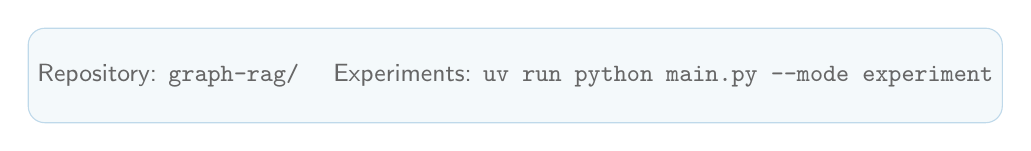
\begin{tikzpicture}
  \node[draw=c1!30,rounded corners=6pt,fill=c1!5,
        minimum width=9cm,minimum height=1.2cm,
        font=\small\sffamily\color{black!60},align=center]
    {Repository: \texttt{graph-rag/} \quad
     Experiments: \texttt{uv run python main.py --mode experiment}};
\end{tikzpicture}
\end{frame}

\end{document}
